\documentclass[journal]{IEEEtran}

% *** CITATION PACKAGES ***
%
%\usepackage{cite}
\usepackage{capt-of}%%To get the caption
\usepackage{gensymb}
\usepackage{graphicx} %package to manage images
\graphicspath{ {./images/} }
\usepackage{wrapfig}

\usepackage{amsmath}
\usepackage{amssymb}


\usepackage[style=ieee]{biblatex}
\DeclareLanguageMapping{english}{english-apa}
\addbibresource{references.bib}
\usepackage[justification=centering]{caption}

\usepackage{setspace}

\usepackage{hhline}


\usepackage{changepage} 

\usepackage{booktabs}
\usepackage{xcolor}

\usepackage{makecell}

\renewcommand\theadfont{}

%\raggedbottom

% *** GRAPHICS RELATED PACKAGES ***
%
\ifCLASSINFOpdf
  % \usepackage[pdftex]{graphicx}
  % declare the path(s) where your graphic files are
  % \graphicspath{{../pdf/}{../jpeg/}}
  % and their extensions so you won't have to specify these with
  % every instance of \includegraphics
  % \DeclareGraphicsExtensions{.pdf,.jpeg,.png}
\else
  % or other class option (dvipsone, dvipdf, if not using dvips). graphicx
  % will default to the driver specified in the system graphics.cfg if no
  % driver is specified.
  % \usepackage[dvips]{graphicx}
  % declare the path(s) where your graphic files are
  % \graphicspath{{../eps/}}
  % and their extensions so you won't have to specify these with
  % every instance of \includegraphics
  % \DeclareGraphicsExtensions{.eps}
\fi
% graphicx was written by David Carlisle and Sebastian Rahtz. It is
% required if you want graphics, photos, etc. graphicx.sty is already
% installed on most LaTeX systems. The latest version and documentation
% can be obtained at: 
% http://www.ctan.org/pkg/graphicx
% Another good source of documentation is "Using Imported Graphics in
% LaTeX2e" by Keith Reckdahl which can be found at:
% http://www.ctan.org/pkg/epslatex
%
% latex, and pdflatex in dvi mode, support graphics in encapsulated
% postscript (.eps) format. pdflatex in pdf mode supports graphics
% in .pdf, .jpeg, .png and .mps (metapost) formats. Users should ensure
% that all non-photo figures use a vector format (.eps, .pdf, .mps) and
% not a bitmapped formats (.jpeg, .png). The IEEE frowns on bitmapped formats
% which can result in "jaggedy"/blurry rendering of lines and letters as
% well as large increases in file sizes.
%
% You can find documentation about the pdfTeX application at:
% http://www.tug.org/applications/pdftex

\begin{document}

\begin{titlepage}
    {\centering
        \vspace*{20em}
        {
        \huge 
        \begin{spacing}{1.5}
            Lab Report \#4: LT Spice Simulation of Transformers
            \\
            Advanced Circuits Lab (ENGR$-$UH 2311),\\
            Spring 2019
            \bigskip
            \Large
            \\
            Transformers and Mutual Inductance in LT Spice
  
            \\
            \bigskip
            Deadline: May 15, 2019 
        \end{spacing}

        }
        
    }
    \vfill
    
    {
    \large
    
    \begin{spacing}{1.5}
    \noindent Barkin Simsek, {\it {bs3528@nyu.edu}} 
    \\
    Nishant Aswani, {\it {nsa325@nyu.edu}}
    \\
    Section \#1% <-this % stops a space
    \\
    Workstation \#8% <-this % stops a space
    \end{spacing}
    }


\end{titlepage}
\pagenumbering{gobble}
%\clearpage\mbox{} % adds and empty page
%\clearpage
\pagenumbering{arabic}
\setcounter{page}{1}

%\title{Demonstration of a Voltage Divider With A Variable Resistor}

%\author{Barkin Simsek,~\IEEEmembership{bs3528@nyu.edu};
%Nishant Aswani,~\IEEEmembership{nsa325@nyu.edu}
%\\ Table Number: \#}% <-this % stops a space


% The paper headers
\markboth{Simsek, Aswani, Advanced Circuits Lab 2019}%
{}

% make the title area
%\maketitle

% As a general rule, do not put math, special symbols or citations
% in the abstract or keywords.
\begin{abstract}
In this lab, the purpose was using the LTSpice software to build and simulate transformers while declaring the mutual inductance between the transformer coils. The voltage and current magnitudes & phase angles were determined by using LTSpice software. The average power dissipated in the load resistor or the second winding was also measured. Measured values were recorded in tables.

\end{abstract}

%%%%%%%%%%%%%%%%%%
%% Introduction %%
%%%%%%%%%%%%%%%%%%
\section{Introduction}

\IEEEPARstart{T}\lowercase{he} concept of mutual inductance is used in transformers, which are used to step up or down AC voltages for transportation purposes. These devices are essentially two coils of wire, inductors, separated by a short distance and operate on the idea of a magnetic flux generated from one coil producing a voltage on the other inductor.

\begingroup
    \centering
    \medskip
    %width=\columnwidth
    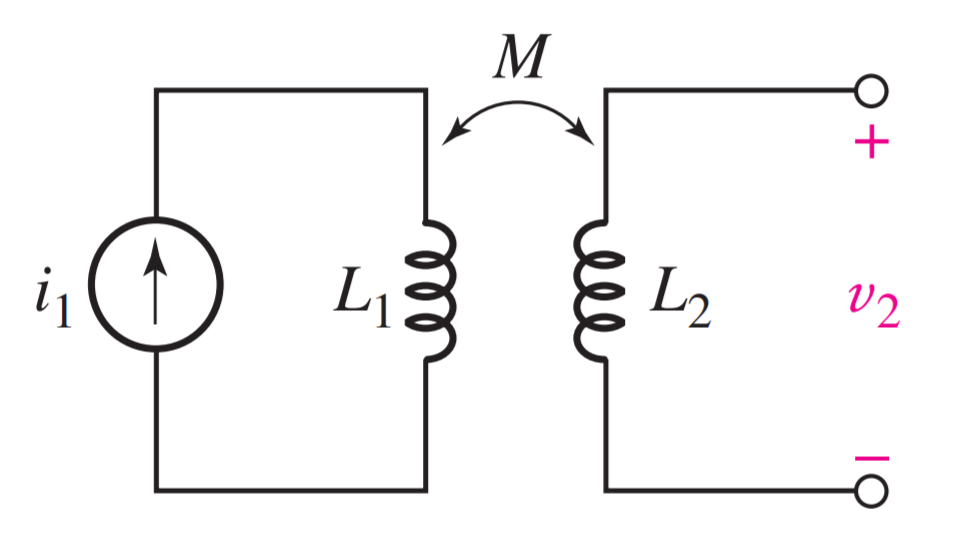
\includegraphics[width=\columnwidth]{images/labx_1.PNG}
    \captionof{figure}{Two inductors separated by a small distance, showing mutual inductance}
    \label{fig:transformer}
    \medskip
\endgroup


\noindent This idea of induced voltage on a nearby coil is called mutual inductance and is quantified by the following equation: 

\begin{equation}
    \begin{split}
        M_{21} & = k \cdot \sqrt{L_{1}L_{2}} \\
       v_{2} & = M_{21}\frac{d_{i1}}{dt}\\
    \end{split}
    \label{eq:mutual}
\end{equation}

\noindent Here, $k$ refers to the coupling coefficient, a constant that is determined by the physical quality of the transformer. A high $k$ is achieved by tighter windings, smaller distances, and a generally concentrated magnetic flux. An ideal transformer is thus defined as a transformer with $k = 1$.

\noindent While $M_{21}$ refers to the mutual inductance on $v_2$ induced by the magnetic flux from $L_1$, there also exists $M_{12}$, which is the mutual inductance by which $L_1$ is affected. The two mutual inductance values are necessarily equal. 

\begingroup
    \centering
    \medskip
    %width=\columnwidth
    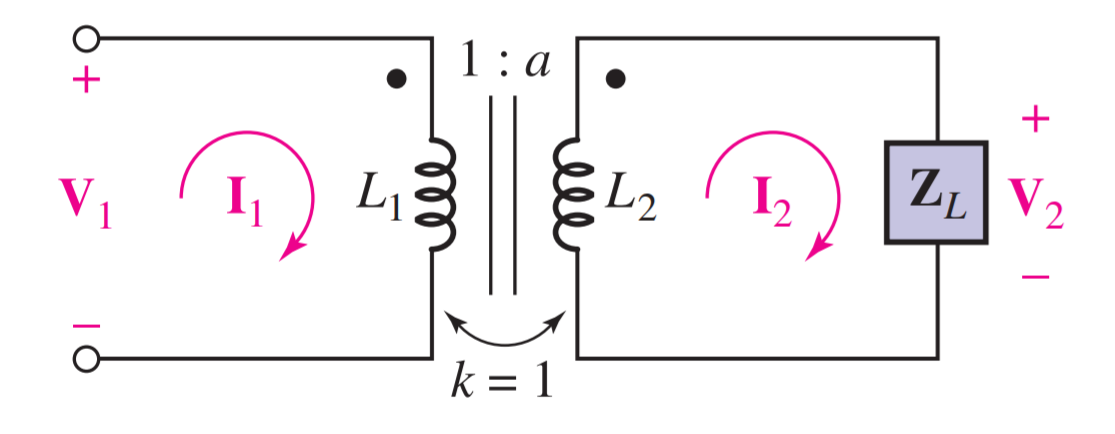
\includegraphics[width=\columnwidth]{images/labx_2.PNG}
    \captionof{figure}{An ideal transformer, denoted by the two parallel lines in between the inductors}
    \label{fig:idealtransformer}
    \medskip
\endgroup

\noindent Ideal transformers also use the concept of the turns ratio. The ratio above the vertical bars refers to the ratio of the number of turns of each inductor coil. 

\begin{equation}
    \begin{split}
        a & = \frac{N_2}{N_1} = \sqrt{\frac{L_2}{L_1}}\\
    \end{split}
    \label{eq:mutual}
\end{equation}

\noindent Other relations in an ideal transformer are also important for several applications and are summarized below.

\begin{equation}
    \begin{split}
        a & = \frac{I_1}{I_2} = \sqrt{\frac{L_2}{L_1}}\\ \\
        a & = \frac{V_2}{V_1} = \sqrt{\frac{L_2}{L_1}}\\
    \end{split}
    \label{eq:mutual}
\end{equation}

\noindent Both the above relations imply that transformers play a role in both current and voltage adjustments. 

\section{Experimental Set-Up}

\noindent Four circuit configurations were created in LT Spice. The first circuit (see Figure \ref{fig:circuit1}), was built using two inductors, a capacitor, a resistor, a voltage source, and three ports to measure voltage.

\begingroup
    \centering
    \medskip
    %width=\columnwidth
    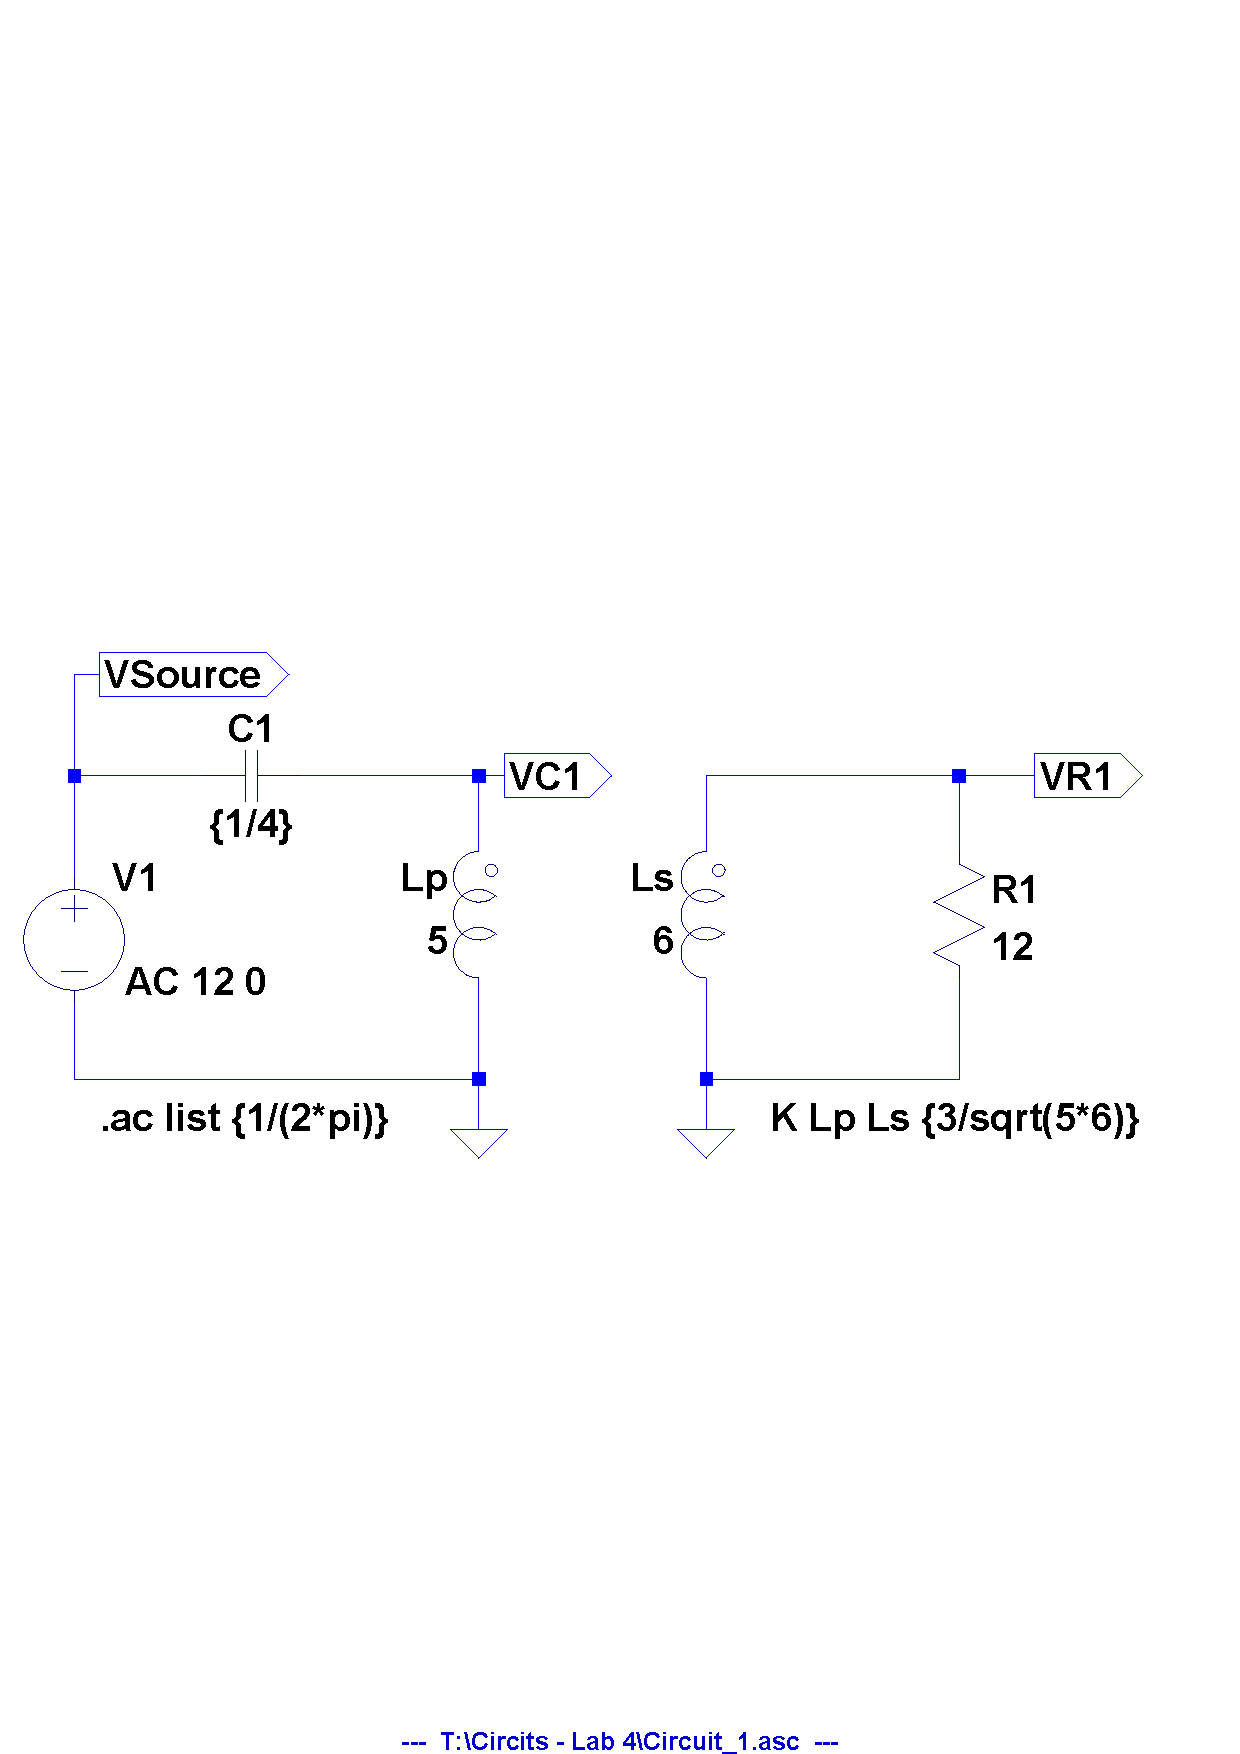
\includegraphics[clip, trim=0.0cm 10cm 0.0cm 10cm, width=\columnwidth]{images/labx_3.pdf}
    \captionof{figure}{Circuit Diagram 1}
    \label{fig:circuit1}
    \medskip
\endgroup

\subsection{Wiring Components}

\noindent All the circuit components (voltage source, capacitor, inductors, and resistor) were laid out on the blank document. Wires were used to connect the poles of each component to resemble two rectangular circuits beside each other. Specifically, each node of the voltage source was connected to a leg of the inductor, with a capacitor in between the wiring in one of the legs. On the other side, the leg of each resistor was wired to the leg of the other inductor. There was no wiring between the two inductors. \\

\noindent From the toolbar, the ground component was selected and connected to the bottom wire on each of the two circuits. The "net" component was also selected, specifying an "out" type, and placing it in three locations: at the positive source terminal, after the capacitor, and before the resistor.

\subsection{Renaming and Assigning Values}

\noindent Each component was appropriately renamed by right-clicking on the default name and relabeling in the pop-up box. Right-clicking on the other label popped-up a larger box, which allowed to change the value of the circuit components. $L_1$ was set to 5 , $L_2$ to 6, $C_1$ to $\frac{1}{4}$, and $R_1$ to 12. Looking at $C_1$'s value reveals that simple functions can be inputted into curly brackets, which LT Spice resolves to specific values. The voltage source was set by setting a 12V to the amplitude in the small AC power analysis section. 

\subsection{Setting the Coupling Coefficient}

\noindent In LT Spice, SPICE directives are texts that are passed onto the netlist, which are scripting descriptions of the circuit. The $k$ value for each of the circuits was set by clicking on the .op tool on the top right. In the pop-up box, the inputted directive was "K Lp Ls \{K\}", where the \{K\} indicates a calculation that resolves to the $k$ value. For example, the K value in Figure \ref{fig:circuit1} was derived as shown in equation \ref{eq:coefficient}:

\begin{equation}
    \begin{split}
        k & = \frac{M}{\sqrt{L_1L_2}} = \frac{3}{\sqrt{5\cdot6}}\\ \\
    \end{split}
    \label{eq:coefficient}
\end{equation}

\subsection{Running the Simulation}\\

\noindent To edit the simulation parameters, "Simulate $\longrightarrow{}$ Edit Simulate Cmd" was selected from the toolbar at the top-left. In the pop-up menu, the "AC Analysis" tab was selected to reveal four parameters and a directive box. The first parameter was selected to be "list" and the desired frequency (60 Hz) was input in the directive box, resulting in ".ac list 60Hz". To run the simulation, "Simulate$\longrightarrow{}$Run" was selected.\\

\noindent The remaining diagrams (Figures \ref{fig:circuit2}, \ref{fig:circuit3}, \ref{fig:circuit4} ) were set-up in a similar way, tweaking parameters specific to the circuits. 

\begingroup
    \centering
    \medskip
    %width=\columnwidth
    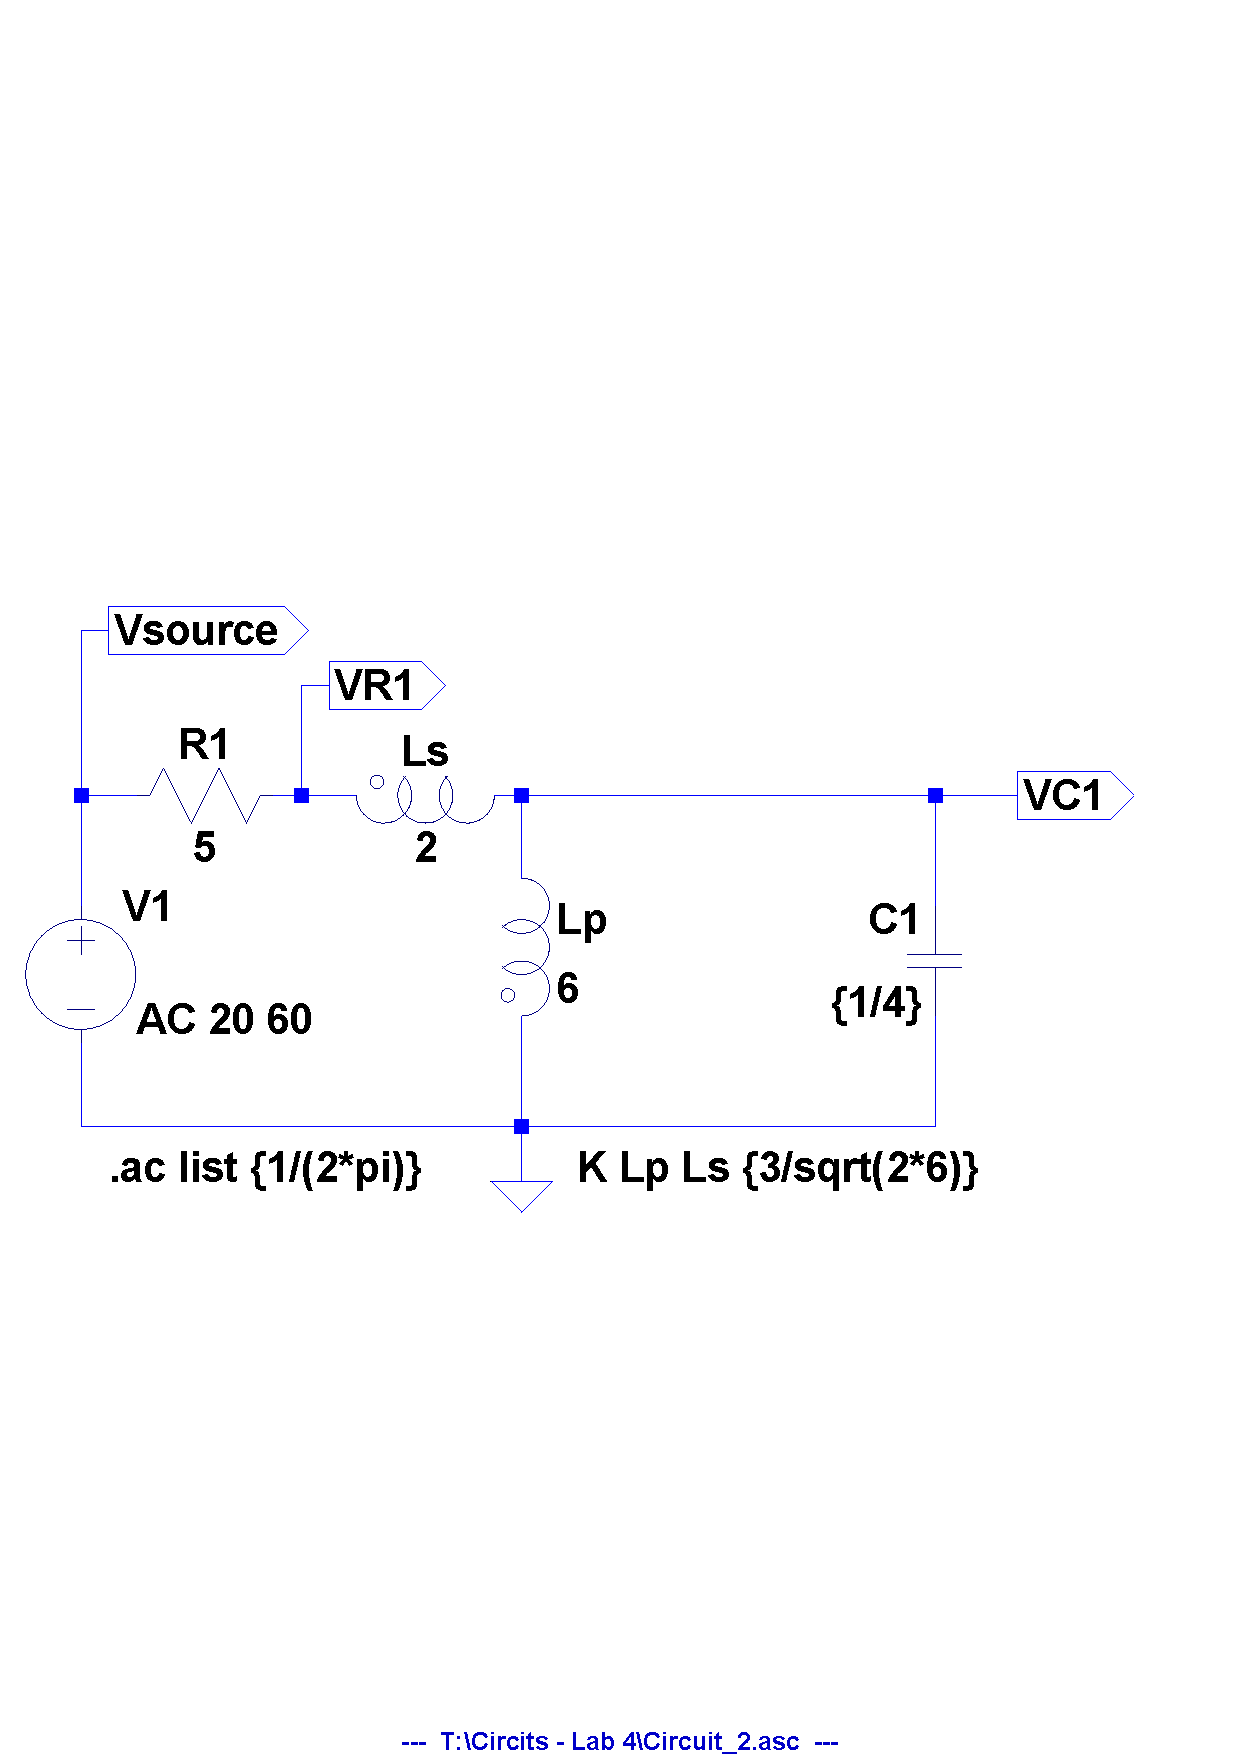
\includegraphics[clip, trim=0.0cm 9cm 0.0cm 9cm, width=\columnwidth]{images/labx_5.pdf}
    \captionof{figure}{Circuit Diagram 2}
    \label{fig:circuit2}
    \medskip
\endgroup

\begingroup
    \centering
    \medskip
    %width=\columnwidth
    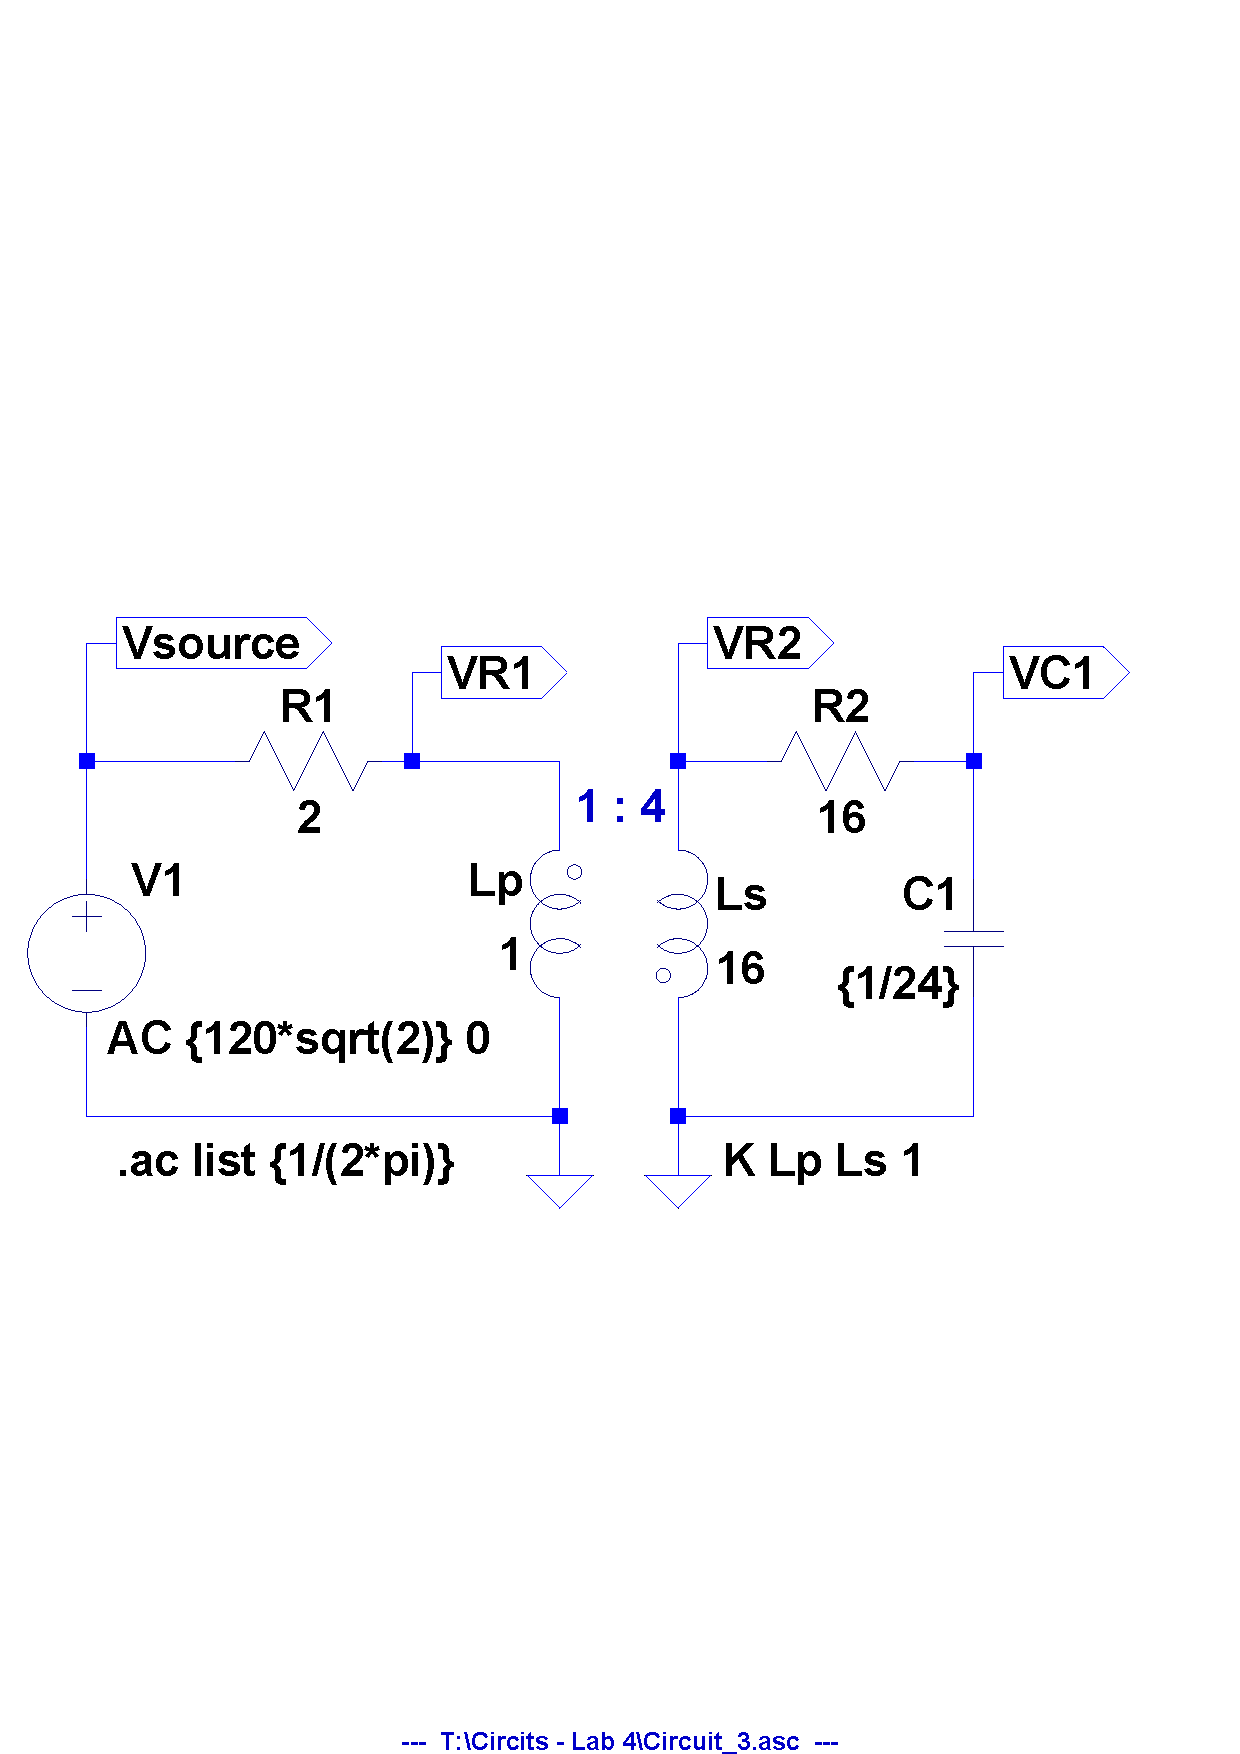
\includegraphics[clip, trim=0.0cm 9cm 0.0cm 9cm, width=\columnwidth]{images/labx_6.pdf}
    \captionof{figure}{Circuit Diagram 3}
    \label{fig:circuit3}
    \medskip
\endgroup

\begingroup
    \centering
    \medskip
    %width=\columnwidth
    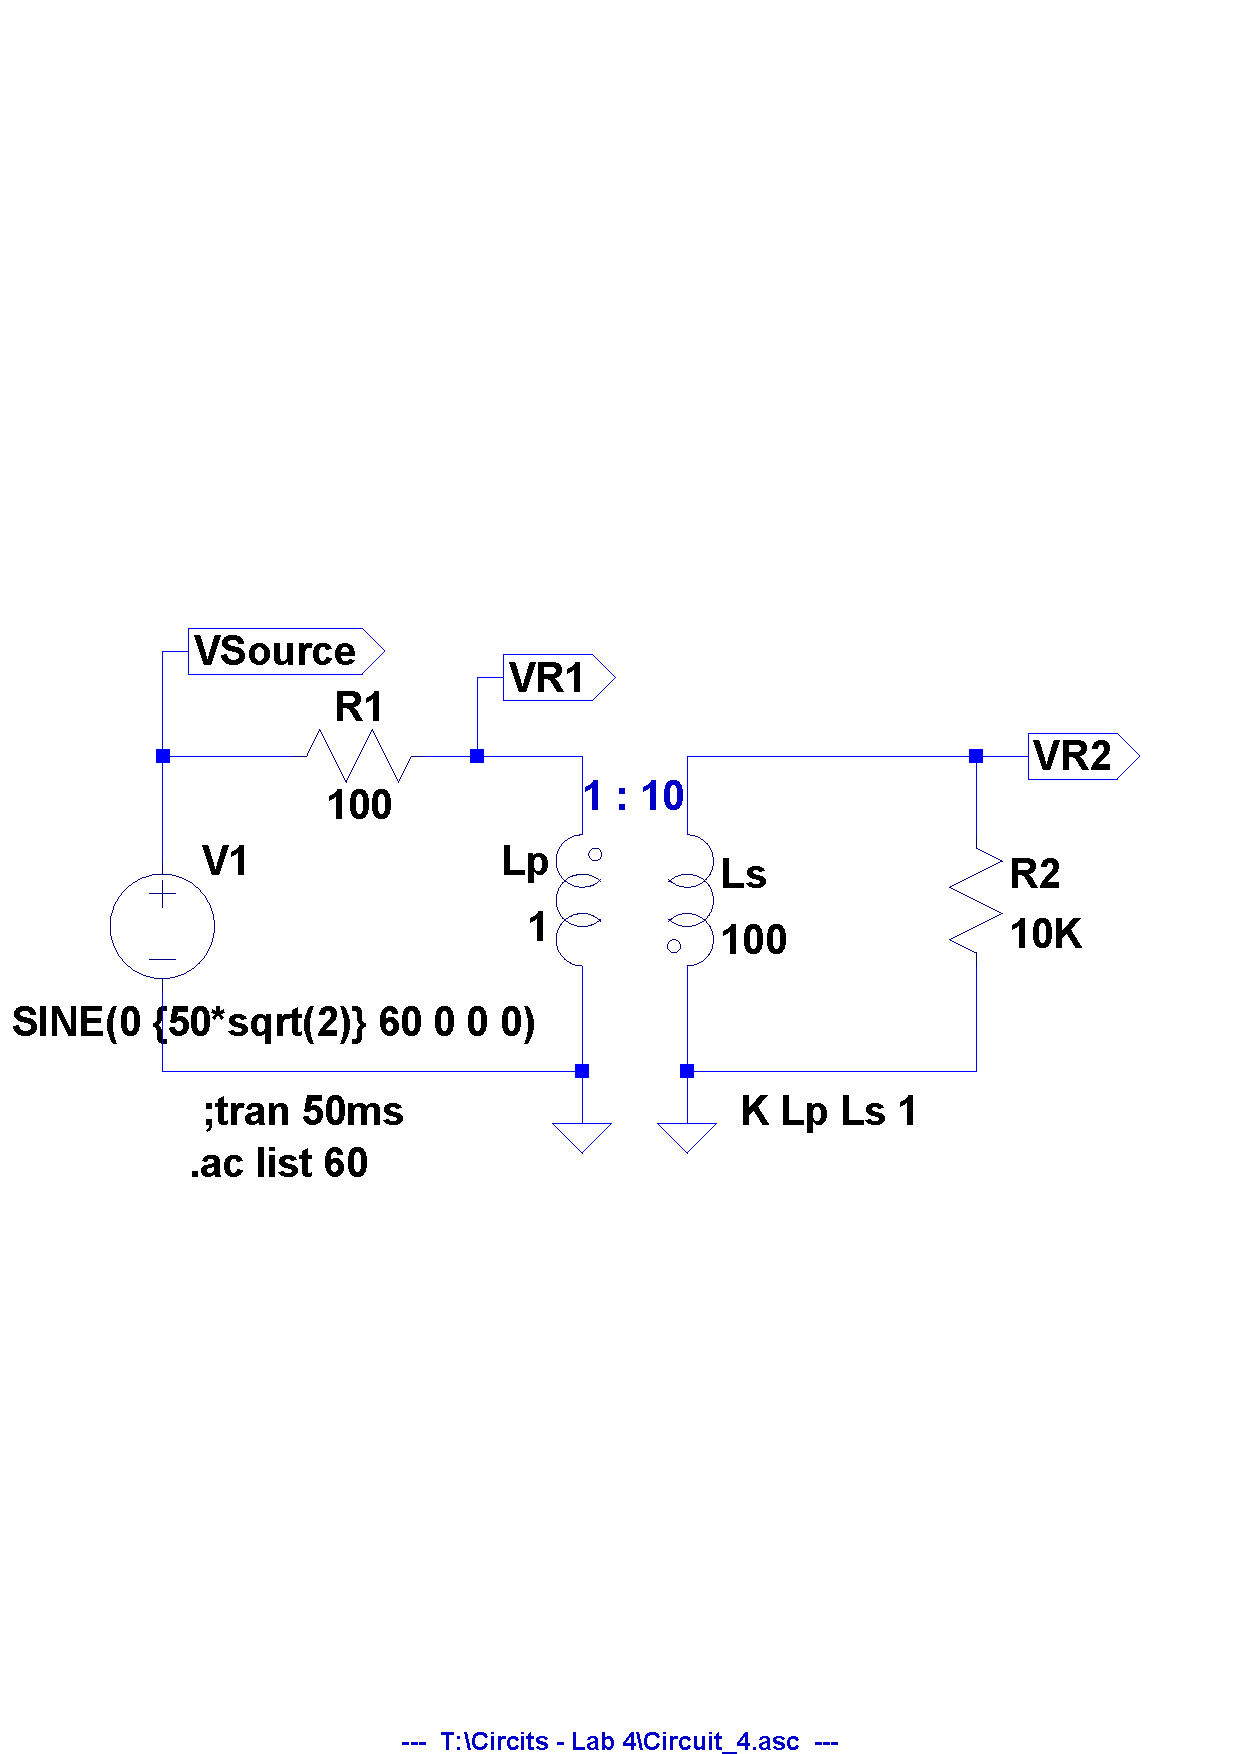
\includegraphics[clip, trim=0.0cm 9cm 0.0cm 9cm, width=\columnwidth]{images/labx_7.pdf}
    \captionof{figure}{Circuit Diagram 4}
    \label{fig:circuit4}
    \medskip
\endgroup

\section{Results and Discussion}

\subsection{Circuit 1}

\noindent The tables below summarizes the simulation results obtained from the first circuit. \\

\begingroup
    \medskip
    \centering
    \def\arraystretch{1.5}
        \begin{tabular}{lcc}
            \toprule
            Source & Voltage (V) & Phase (\degree)\\
            \midrule
            ${C1}$ & 61.6709 & 33.3263\degree\\
            ${R1}$ & 34.9251 & 14.0362\degree\\
            ${Vsource}$ & 12 & 0\degree\\
            \bottomrule
        \end{tabular}
    \captionof{figure}{Circuit 1 voltage results at 0.159155 Hz}
    \label{fig:c1table1}
    \medskip
\endgroup

\begingroup
    \medskip
    \centering
    \def\arraystretch{1.5}
        \begin{tabular}{lcc}
            \toprule
            Source & Current (A) & Phase (\degree)\\
            \midrule
            ${C1}$ & 13.0158 & 130.601\degree\\
            ${Ls}$ & 2.91043 & 14.0362\degree\\
            ${Lp}$ & 13.0158 & 130.601\degree\\
            ${R1}$ & 2.91043 & 14.0362\degree\\
            ${V1}$ & 13.0158 & 130.601\degree\\
            \bottomrule
        \end{tabular}
    \captionof{figure}{Circuit 1 current results at 0.159155 Hz}
    \label{fig:c1table2}
    \medskip
\endgroup

\noindent Most obviously, there was a 12V drop across $V_{1}$, as shown by the $v_{source}$ measurement, with no change in phase angle. $v_{c1}$ shows the voltage drop across the inductor, which had a phase angle of approximately 33\degree. The positive phase angle provides a simple confirmation of the inducing nature of the component. The phase angle seen in $v_{r1}$, in the secondary coil, is equivalent to the phase angle of the current, once again confirming that resistors do not cause any phase shifts in the circuit. \\

\noindent The equations below summarize a mesh analysis of the mutually coupled inductors.\\


Primary loop:

\begin{equation}
    \begin{split}
        0 & = -12\angle0\degree + -j4(I_{1}) + j5(I_{1}) -j3(I_{2})\\
    \end{split}
    \label{eq:primary}
\end{equation}

Secondary loop:

\begin{equation}
    \begin{split}
        0 & = j6(I_{2}) + 12(I_{2}) -j3(I_{1})\\
    \end{split}
    \label{eq:secondary}
\end{equation}

Solving this system of equations provides $I_{1}$ to be $13.01\angle-49.40\degree$ and $I_{2}$ to be $2.91\angle14.04\degree$, results alike to the ones from the simulations.

\subsection{Circuit 2}

\noindent The simulation results from circuit 2 are summarized below. 

\begingroup
    \medskip
    \centering
    \def\arraystretch{1.5}
        \begin{tabular}{lcc}
            \toprule
            Source & Voltage (V) & Phase (\degree)\\
            \midrule
            ${C1}$ & 21.4663 & -3.43495\degree\\
            ${R1}$ & 8.94427 & -3.43495\degree\\
            ${Vsource}$ & 20 & 60\degree\\
            \bottomrule
        \end{tabular}
    \captionof{figure}{Circuit 2 voltage results at 0.159155 Hz}
    \label{fig:c2table1}
    \medskip
\endgroup

\begingroup
    \medskip
    \centering
    \def\arraystretch{1.5}
        \begin{tabular}{lcc}
            \toprule
            Source & Current (A) & Phase (\degree)\\
            \midrule
            ${C1}$ & 5.36656 & -93.4349\degree\\
            ${Ls}$ & 3.57771 & -93.4349\degree\\
            ${Lp}$ & 1.78885 & -93.4349\degree\\
            ${R1}$ & 3.57771 & -93.4349\degree\\
            ${V1}$ & 3.57771 & -93.4349\degree\\
            \bottomrule
        \end{tabular}
    \captionof{figure}{Circuit 2 current results at 0.159155 Hz}
    \label{fig:c2table2}
    \medskip
\endgroup

\noindent Looking at Figure \ref{fig:circuit2}, it is clear that the mutually coupled inductors are in series with one other. Aside from the evident $v_{source}$ measurement, the circuit displays another obvious result: the Kirchoff's node law at the action. The magnitude of the current flowing through the resistor and secondary inductor, when added to the magnitude of the current flowing through the primary inductor, results in the magnitude of the current flowing through the capacitor.\\ 

\noindent Comparing  $v_{r1}$ and  $v_{c1}$, it becomes clear that there is a difference in magnitude but equivalence in phase. Given that $I_{1}$ is equal to $3.57\angle-93.43\degree$ and $I_{2}$ is equal to $1.79\angle-93.43\degree$, calculating these values is a simple application of Ohm's law. In the case of $v_{r1}$, it is done so by adding the voltage drops across the two inductors, or across $L_{s}$ and the capacitor. It is by coincidence that phase angle across the two voltage measurements is equivalent. 

\subsection{Circuit 3}

\noindent The tables below summarize the simulation output from circuit 3. 

\begingroup
    \medskip
    \centering
    \def\arraystretch{1.5}
        \begin{tabular}{lcc}
            \toprule
            Source & Voltage (V) & Phase (\degree)\\
            \midrule
            $V_{Vr1}$ & 87.4118 & 33.6901\degree\\
            $V_{Vr2}$ & 349.647 & -146.31\degree\\
            $V_{Vsource}$ & 169.706 & 0\degree\\
            $V_{Vc1}$ & 290.924 & -180\degree\\
            \bottomrule
        \end{tabular}
    \captionof{figure}{Circuit 3 voltage results at 0.159155 Hz}
    \label{fig:c3table1}
    \medskip
\endgroup

\begingroup
    \medskip
    \centering
    \def\arraystretch{1.5}
        \begin{tabular}{lcc}
            \toprule
            Source & Current (A) & Phase (\degree)\\
            \midrule
            ${C1}$ & 12.1218 & 90\degree\\
            ${Ls}$ & 12.1218 & 90\degree\\
            ${Lp}$ & 54.2105 & 153.435\degree\\
            ${R1}$ & 54.2105 & 153.435\degree\\
            ${R2}$ & 12.1218 & -90\degree\\
            ${V1}$ & 54.2105 & 153.435\degree\\
            \bottomrule
        \end{tabular}
    \captionof{figure}{Circuit 3 current results at 0.159155 Hz}
    \label{fig:c3table2}
    \medskip
\endgroup

As the voltage source provided for this circuit was a root-mean-square value, it had to be converted to the peak to peak voltage by scaling it by a factor of $\sqrt{2}$. As this circuit has a similar configuration to the first circuit, a similar analytical method can be applied to retrieve the simulation results. For simplicity, the primary inductor was chosen to have an inductance of 1, making the calculation for the secondary inductor quite simple. The secondary inductance value was calculated using the following relation, where a is the turns ratio: 

\begin{equation}
    \begin{split}
        a & = \sqrt{\frac{Z_p}{Z_s}}\\
    \end{split}
    \label{eq:turns}
\end{equation}

\captionof{figure}{Circuit 4 results}

\noindent The results of the final simulation are as follows: 

\begingroup
    \medskip
    \centering
    \def\arraystretch{1.5}
        \begin{tabular}{lcc}
            \toprule
            Source & Voltage (V) & Phase (\degree)\\
            \midrule
            ${Vr1}$ & 35.0484 & 7.555\degree\\
            ${Vr2}$ & 350.484 & -172.445\degree\\
            ${Vsource}$ & 70.7107 & 0\degree\\
            \bottomrule
        \end{tabular}
    \captionof{figure}{Circuit 4 voltage results at 60 Hz}
    \label{fig:c4table1}
    \medskip
\endgroup

\begingroup
    \medskip
    \centering
    \def\arraystretch{1.5}
        \begin{tabular}{lcc}
            \toprule
            Source & Current (A) & Phase (\degree)\\
            \midrule
            ${Ls}$ & 0.0350484 & 7.555\degree\\
            ${Lp}$ & 0.362605 & 172.699\degree\\
            ${R1}$ & 0.362605 & 172.699\degree\\
            ${R2}$ & 0.0350484 & -172.445\degree\\
            ${V1}$ & 0.362605 & 172.699\degree\\
            \bottomrule
        \end{tabular}
    \captionof{figure}{Circuit 4 current results at 60 Hz}
    \label{fig:c4table2}
    \medskip
\endgroup

\noindent The average power through the $10k\ohm$ resistor was also found using the simulation and the value obtained can be seen in Figure \ref{fig:avgpower}. 

\begingroup
    \centering
    \medskip
    %width=\columnwidth
    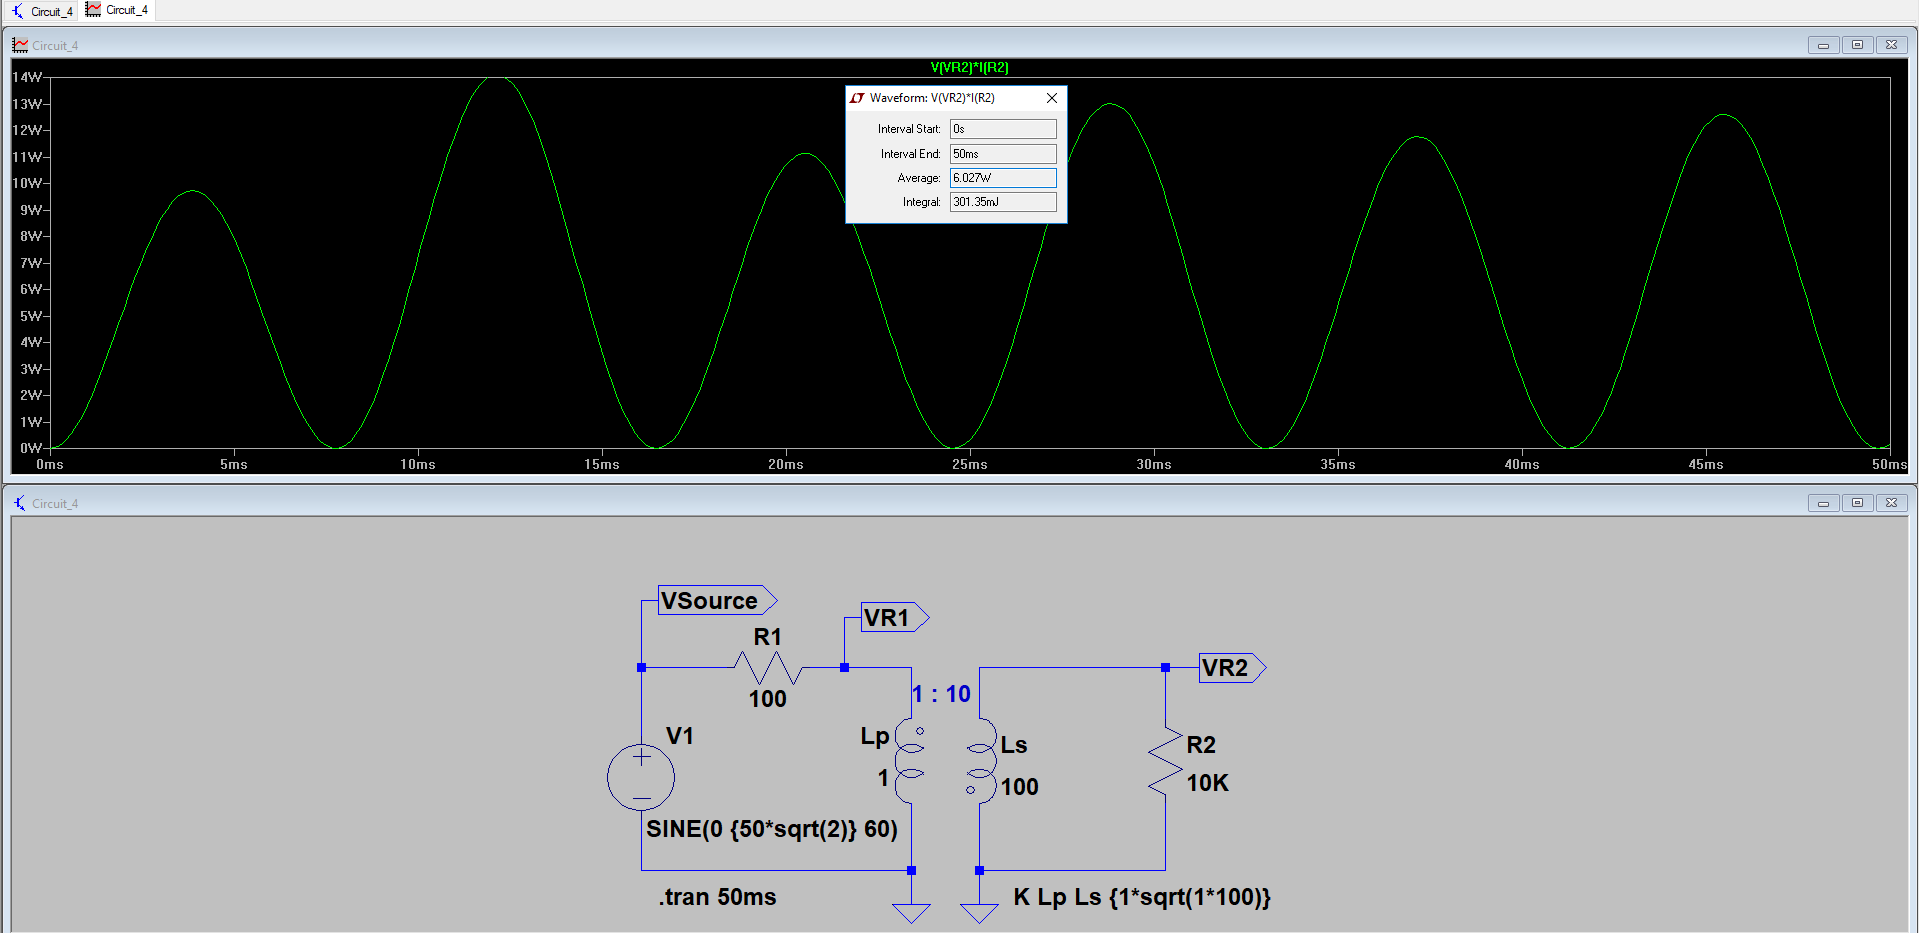
\includegraphics[width=\columnwidth]{images/labx_8.png}
    \captionof{figure}{Circuit Diagram 4}
    \label{fig:avgpower}
    \medskip
\endgroup

\noindent Referring back to Figure \ref{fig:c3table}, calculating the power should be a simple matter of multiplying  $V_{r2}$ by  $I_{r2}$. however, doing so results in the value $12.284\angle15.11\degree$, which has a magnitude roughly double to the 6.03W provided in the simulation.\\

\noindent This discrepancy in results can be explained by inconsistency in using $V_{rms}$ and $V_{m}$. When using the values from the table to calculate power, the equation used should be $\frac{V_{m}I{m}}{2}$. Essentially, a simple multiplication of the values, as was done above, incorrectly assumes that values used are RMS values. The simulation, however, accounts for this and thus uses the correct method to obtain the average power. 

\section{Conclusion}

\noindent Simulating mutually coupled inductors in LT Spice brought a deeper understanding of how the software operates. The use of SPICE directives was brought into the light, as a valuable tool to define constraints and parameters for the circuit, especially more arbitrary ones such as mutual inductance and coupling coefficients. As was the case in the previous lab, this lab also demonstrated some of the measures the software takes to ensure a correct answer, making it a valuable tool. 

\noindent In the future, it would benefit from gaining a more nuanced understanding of the analyses tools, such as the difference and purpose behind using a small signal AC analysis or a standard sinusoidal analysis. It would also be interesting to explore how far the SPICE directives can be taken in describing a circuit, and whether a circuit can be built purely out of these directives. 





\noindent



\printbibliography

\end{document}